\documentclass[12pt,a4paper,twoside]{article}

\usepackage[utf8]{inputenx}
\usepackage[T1]{fontenc}
\usepackage[spanish]{babel}

\usepackage{amsmath}
\usepackage{ifpdf}
\ifpdf
\usepackage{graphicx}
\else
\usepackage[dvipdfmx]{graphicx}
\fi

\usepackage{lipsum}



\title{Practicando con \TeX4ht{}}
\author{Eva María Mazcuñán Navarro}

\begin{document}

\maketitle

%\tableofcontents

\section{Matemáticas}
Veamos cómo se visualizan en el navegador:

\begin{itemize}
	\item las fórmulas delimitadas con dólares $1<x<2$, $x^2+y^2=9$ y $y=\sqrt{9-x^2}$
	
	\item las fórmulas delimitadas con paréntesis \(1\le x \le 2\), \(x^2+y^2=9\) y  \(y=\sqrt{9-x^2}\)
	
	\item la fórmula \[\int_a^b f(x)dx.\]
\end{itemize}

\section{Imágenes}

\noindent Lorem ipsum dolor sit amet, consectetuer adipiscing elit.\\
\noindent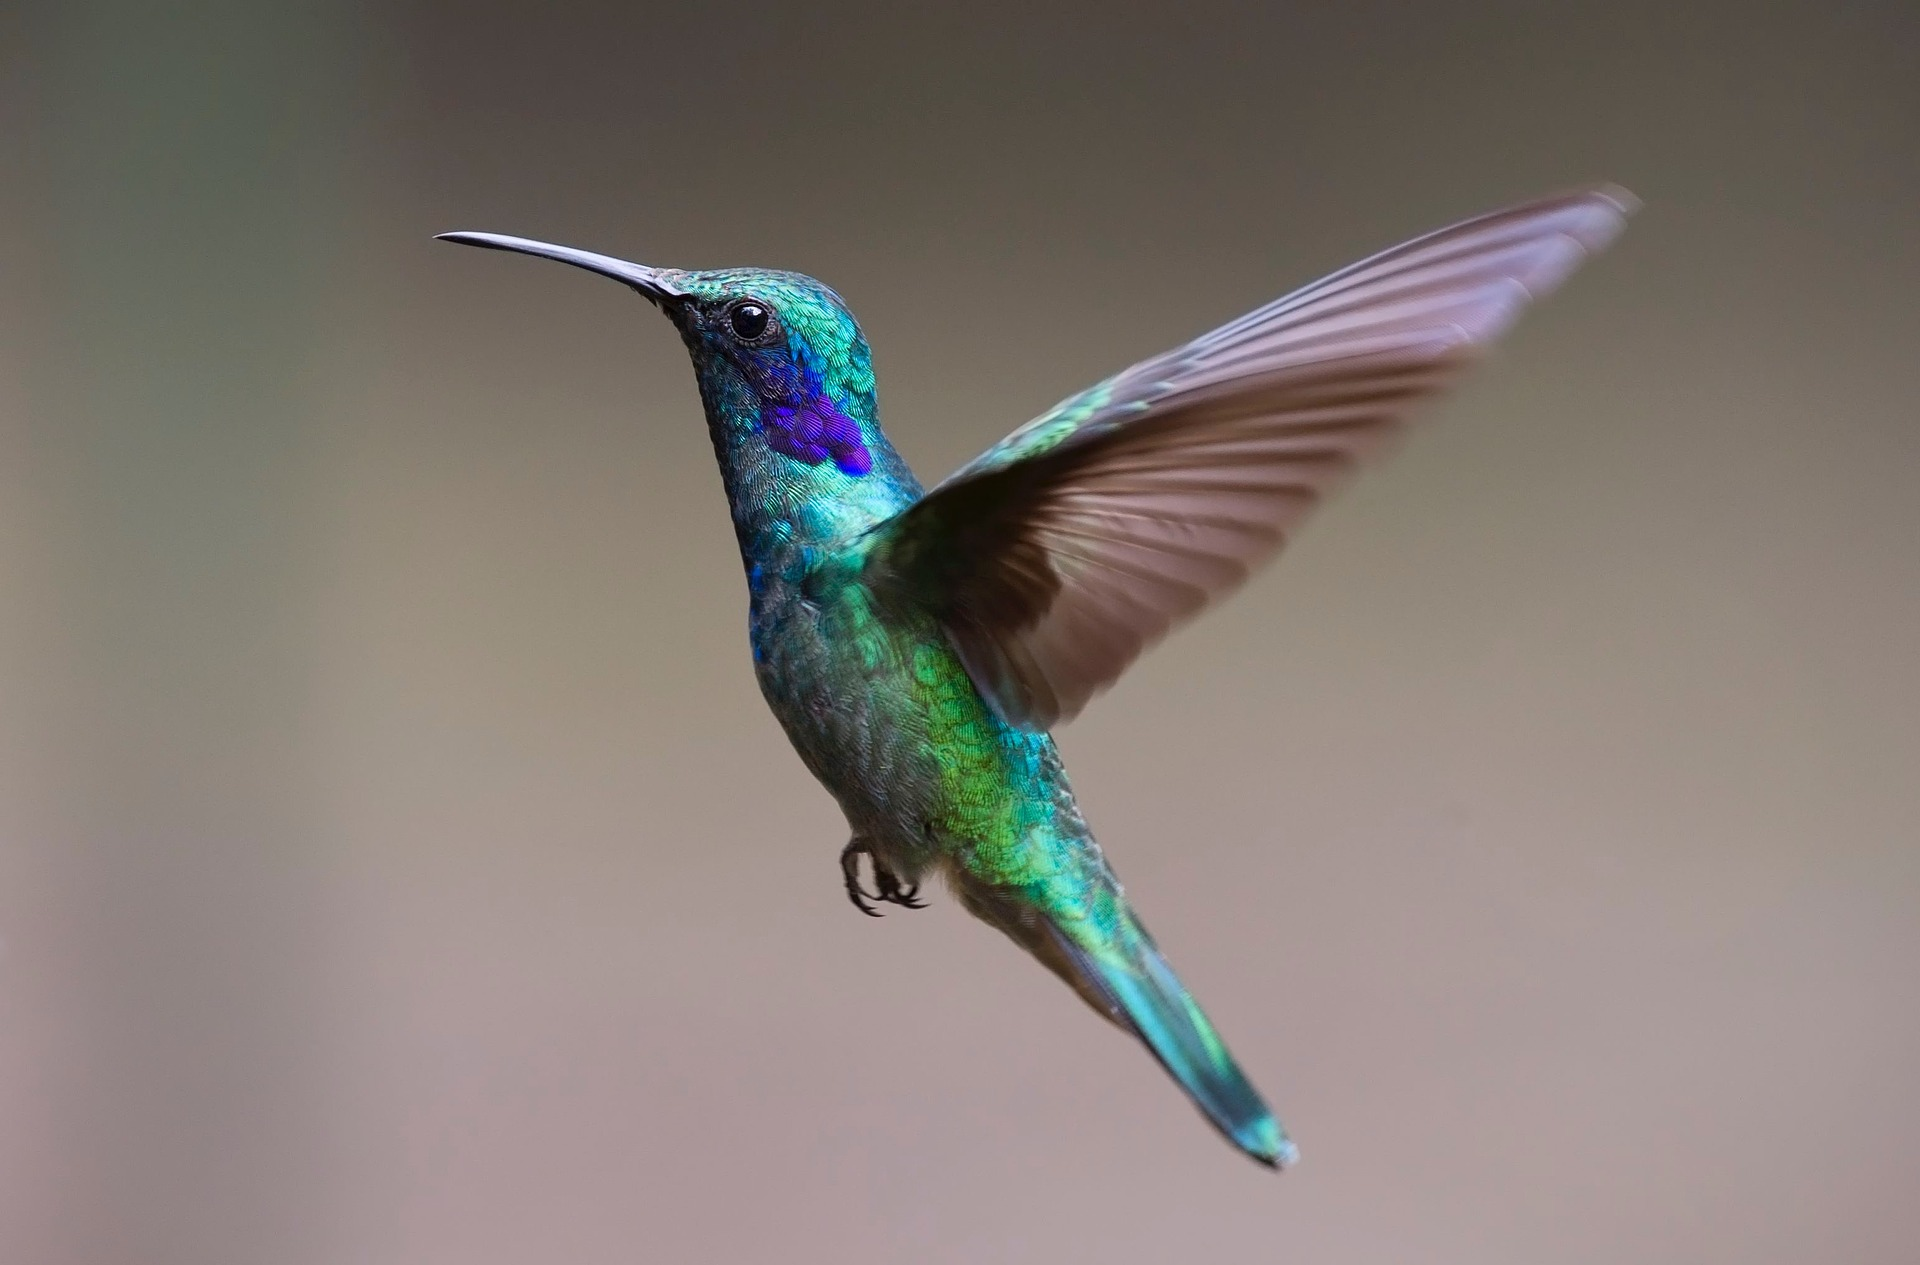
\includegraphics[width=.4\textwidth]{images/bird.jpg}\\
\noindent Lorem ipsum dolor sit amet, consectetuer adipiscing elit.\\
\noindent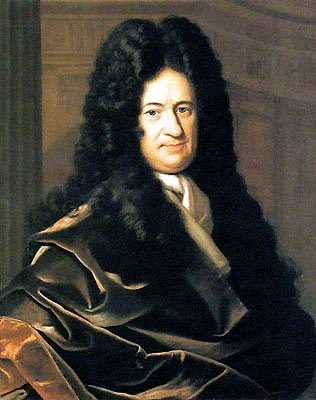
\includegraphics[width=.4\textwidth]{images/GWLeibniz.png}

\noindent Lorem ipsum dolor sit amet, consectetuer adipiscing elit.\\
\noindent\rule[2mm]{4cm}{3mm}\\
\noindent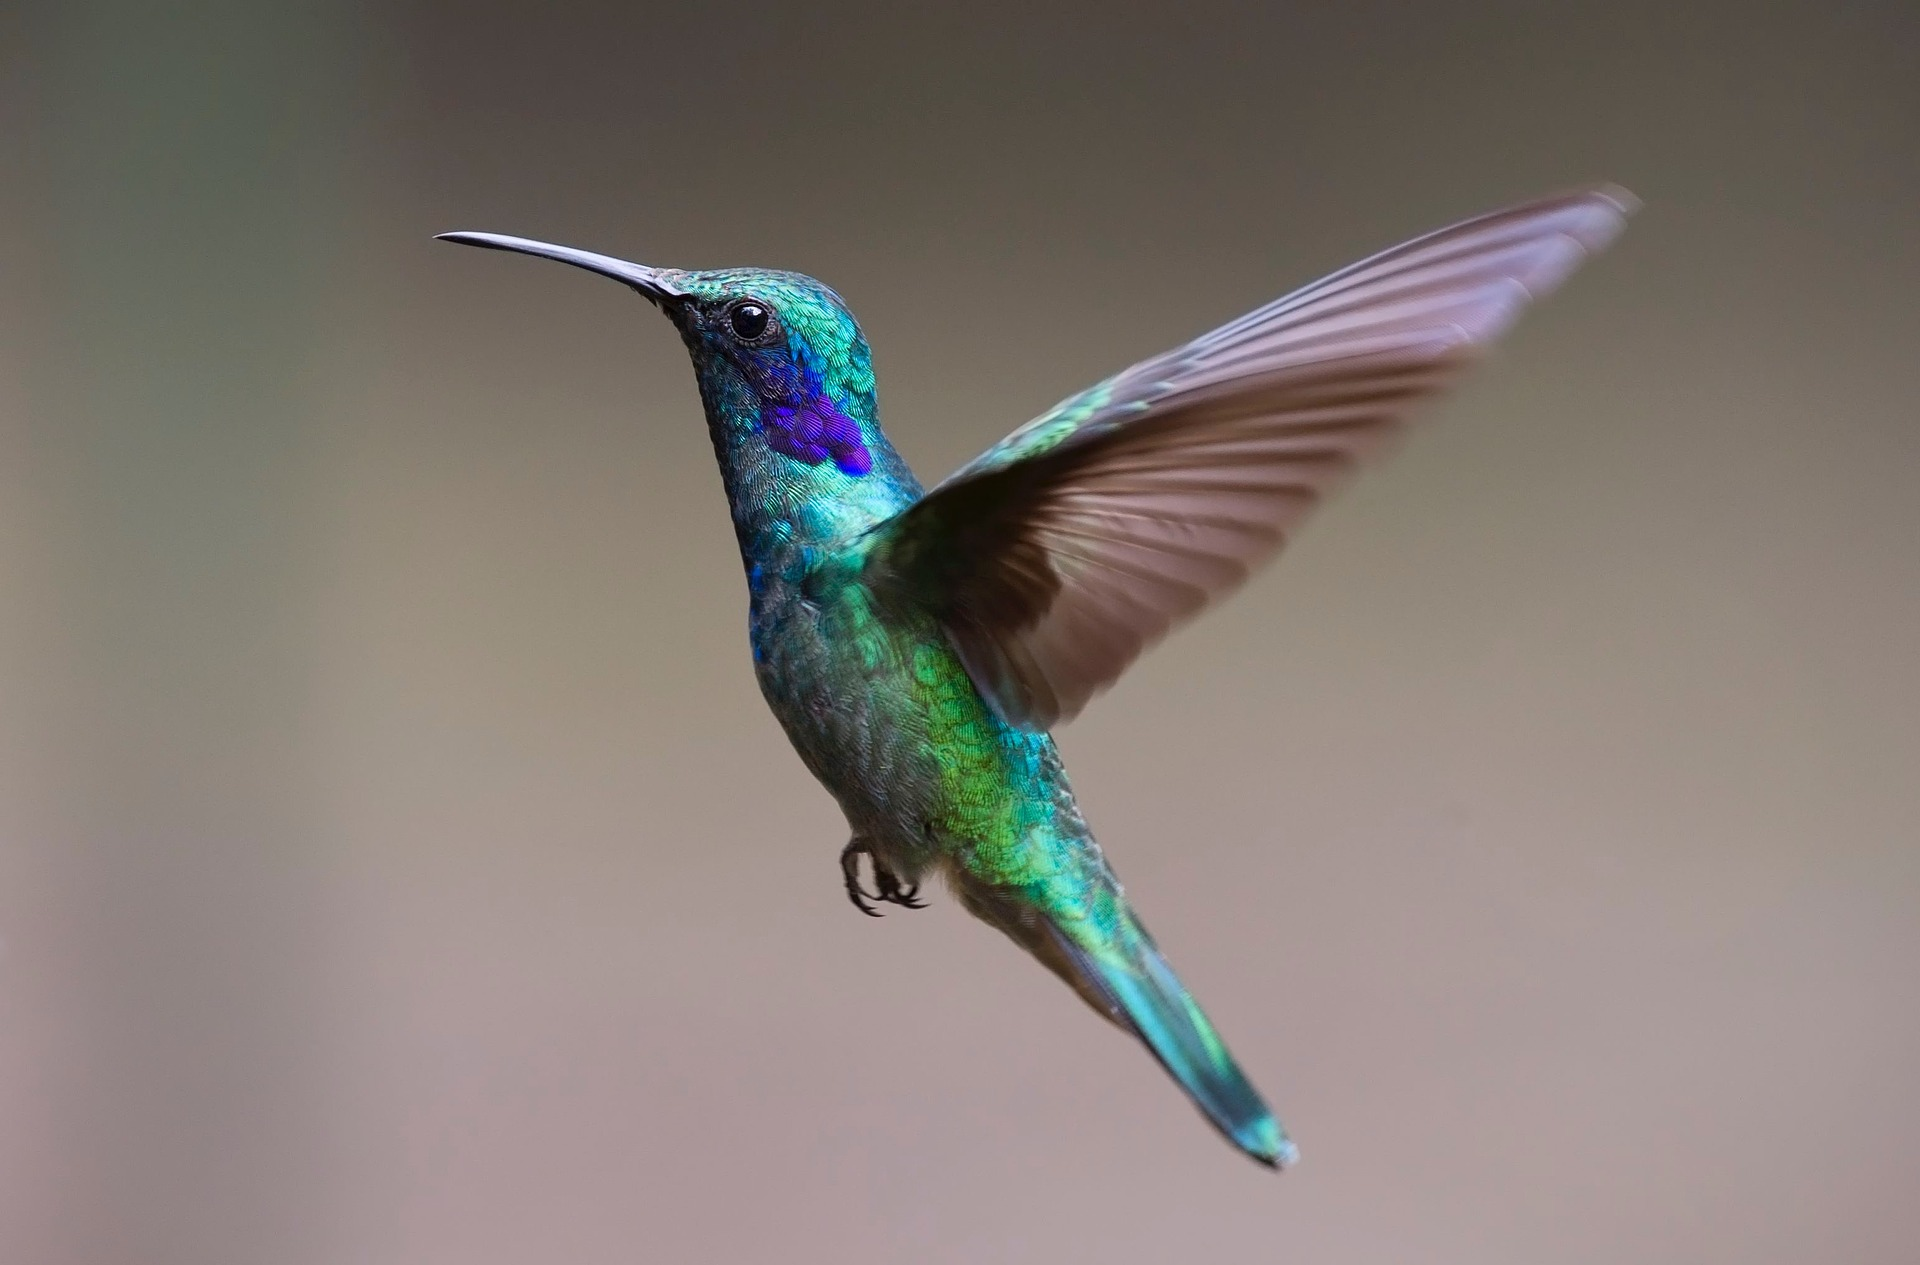
\includegraphics[width=4cm]{images/bird.jpg}\\
\noindent Lorem ipsum dolor sit amet, consectetuer adipiscing elit.\\
\noindent\rule[10pt]{4cm}{3mm}\\
\noindent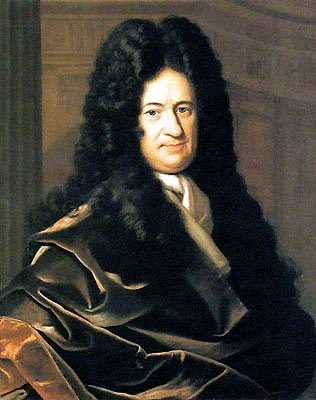
\includegraphics[width=4cm]{images/GWLeibniz.png}




\section{Sección de relleno}

\lipsum[1-15]

\subsection{Subsección}

\lipsum[1-15]

\subsection{Otra subsección}

\lipsum[1-15]		

\section{Otra sección de relleno}

\lipsum[1-15]		

\section{Una última sección de relleno}

\lipsum[1-15]

\end{document}